
\documentclass{stat572Style}
\usepackage{natbib}
\usepackage{amssymb}
\usepackage{graphicx}
\usepackage{amsmath}
%%\setlength{\oddsidemargin}{0.25in}
%%\setlength{\textwidth}{6in}
%%\setlength{\topmargin}{0.5in}
%%\setlength{\textheight}{9in}

\renewcommand{\baselinestretch}{1.5} 

\bibliographystyle{plainnat}

\begin{document}
%%\maketitle

\begin{center}
  {\LARGE A Review of Lagrangian Time Series Models for Ocean Surface Drifter Trajectories (Sykulski et al. (2016))}\\\ \\
  {Hannah Director \\ 
    Department of Statistics, University of Washington Seattle, WA, 98195, USA
  }
\end{center}



\begin{abstract}
  This report reviews the spectral analysis method for modeling ocean surface drifters proposed by \citet{Sykulski2016}. Previous methods to model drifters are discussed along with the authors' model.   Where relevant to understanding the model of \citet{Sykulski2016},  spectral analysis, Mat\'{e}rn covariances, the complex Ornstein-Uhlenbeck process, and Whittle likelihood are reviewed.  To conclude the review, we evaluate the strengths and weaknesses of this method. 
  \end{abstract}

\section{Introduction}
\indent ``Lagrangian Time Series Models for Ocean Surface Drifter Trajectories," by Adam M. Sykulski, Sofia C. Olhede, Jonathan M. Lilly, and Eric Danioux presents a multi-component spectral model for analysis of data transmitted by ocean surface drifters. Drifters are free-floating  instruments that transmit their location at regular time intervals,  creating a \textbf{\it{Langrangian time series}}, or a sequence of spatial locations over time. Oceanographers use these time series to increase understanding of  ocean circulation patterns. Published in January 2016 in the \textbf{\it{Journal of the Royal Statistical Society Series C}}, this paper develops a model that can isolate a scientific quantity of interest,  and, in so doing, introduces several new statistical techniques.\\
\indent The motion of parcels of water moving over changing latitudes is known to have a rotational component. Because the Earth has  different diameter at different latitudes, the speed of objects moving with Earth's rotation varies across latitudes.  This induces a phenomena known as the Coriolis Effect, whereby very fast moving objects or objects being observed over long periods, such as drifters, end up moving at speeds that are different than the Earth beneath them as they change latitude. Viewed from a stationary reference frame, this creates circular motions, or inertial oscillations. These motions have known frequencies, referred to as inertial frequencies. Oceanographers  are interested in detecting deviations from these frequencies, as they are thought to indicate eddies, or persistent circular wave patterns \citep{Kunze1985}. However, the ocean has a constant turbulent background flow which makes identifying eddies in real data difficult \citep{ Elipot2010}. Previous methods to model drifters are BLAH The methods in this paper overcome this challenge and successfully find shifts in the inertial frequency with a spectral time series model. \\
\indent In achieving this result, several statistical advances are made.  The authors introduce an additive spectral domain model that has components corresponding to both the turbulent background and the inertial oscillations. For the turbulent background model, the Mat\'{e}rn covariance commonly used in spatial statistics \citep{Gneiting2012} is extended to the time-series context. This allows for a more flexible model for background behavior than previously obtained.  Inertial oscillations are modeled with a complex Ornstein-Uhlenbeck (OU) \citep{Arato1962, Jeffreys1968}, which provides a stochastic equivalent to an accepted set of coupled differential equations describing inertial oscillations. Further statistical innovation is employed in fitting the model with a variation on standard Whittle likelihood that reduces bias. Time-varying parameter estimates are also introduced to allow for non-stationarity.  \\
\indent The remainder of this review proceeds as follows. After a succinct review of spectral analysis, Section 2 discusses the model for the drifters and the methods used to fit it. Section 3 presents the paper's results including analysis of a long time series with time-varying parameters and an application from a simulated model. Section 4 concludes the review with a discussion of the value and limitations of the approach taken by \citet{Sykulski2016}. 
\section{Methods}
			

	\subsection{Spectral Analysis}
	\label{sec: specAnalysis}
	\indent We briefly review spectral analysis as these methods are central to understanding \citet{Sykulski2016}.  More thorough coverage of this material can be found in  \citep{Percival1993}, for example. From a statistical perspective, a time series, $z(t)$, real or complex-valued,  can be understood as a realization of a stochastic process over time, where  $t = \{1,2,...,n\}$ are the observed time points.  Time series are often modeled as the sums of periodic functions, which, using Euler's formula, can be represented compactly as Fourier series. Moreover, data in the time domain can easily be related to data in the frequency domain and vice versa using the Fourier or inverse Fourier transformations 	\begin{align}
z(t) = \int_{-\infty}^{\infty} f_{z}(\omega)e^{i\omega t}d\omega && f_{z}(\omega) = \int_{-\infty}^{\infty} z(t) e^{-i \omega t }dt.
\end{align}
\citep{Percival1993}. To understand the distribution of frequencies, the \textbf{\it{power spectral density}},
\begin{equation}
S_{z}(\omega) = \underset{T \rightarrow \infty}{\lim} \mathbb{E} \left(\frac{1}{2T} \left| \int_{-T}^{T} z(t) e^{-i \omega t}dt \right|^{2} \right),
\end{equation}
is often employed. This quantity represents the variance (or power) associated with each frequency \citep{Percival1993}. Power spectral densities are useful for statistical modeling, since they can be related to the autocovariance sequence of a time series using  Fourier transformation.  For real $z(t)$, we define the autocovariance as $s_{x}(\tau) = \mathbb{E}[z(t) z(t - \tau)] $ and for complex $z(t)$, we define $s_{x}(\tau) = \mathbb{E}[z(t) z^{*}(t - \tau)] $ where $z^{*}(t)$ represents the complex conjugate of z(t). Letting $\tau$ is the time lag, we have
\begin{align}
\label{eq: fourierPair}
S_{z}(\omega) = \int_{-\infty}^{\infty}s_{z}(\tau) e^{-\omega t}dt  \Longleftrightarrow s_{x}(\tau) = \frac{1}{2\pi} \int_{-\infty}^{\infty}S_{z}(\omega) e^{i \omega t} d\omega 
\end{align}

\noindent \citep{Sykulski2013}. For an observed time series, the power spectral density is often estimated with the periodogram, $\hat{S}_{x}(\omega) = |J_{x}(\omega)|^{2}$ where 
\begin{equation}
\label{eq: perio}
J_{x}(\omega) = \sqrt{\frac{t}{N}} \sum_{t=1}^{N} x(t) e^{-i \omega t}
\end{equation}
\citep{Sykulski2013}. Although intuitively appealing, this estimator has known problems that stem from   sampling a periodic function at discrete intervals. In particular,  high frequencies can  capture periodic behavior of other lower frequencies if that happen to align in period. Additionally, frequencies above the highest observable frequency cannot be captured, and, are instead, recorded as other frequencies in the spectrum.  These effects, referred to as $\textbf{\it{aliasing}}$ and $\textbf{\it{leakage}}$ respectively,  are typically reduced by $\textbf{\it{tapering}}$. This method uses  a window of frequencies for estimation rather than a single value. However, depending on how tapering is used, it can introduce its own  biases in estimation.  


\subsection{Stochastic Model}
 To model the drifters' motions over time, the eastward and northward components of the drifters' velocities, denoted $u(t)$ and $v(t)$ respectively, are converted to a complex-valued velocity, $z(t) = u(t) + iv(t)$. Separate stochastic models are introduced for the inertial oscillation and turbulent background components of the drifter's behavior. Working in the frequency domain, the two components of the model are added together, creating a six-parameter spectral model. Parameter estimates for this model are obtained via maximizing the model's blurred Whittle likelihood, a relatively new approximation to the true spectral likelihood that balances computational efficiency with minimizing bias \citep{Sykulski2013}. 
 
\subsubsection{Inertial oscillations}
We begin by discussing the model for the inertial oscillations. In a deterministic setting, inertial oscillations are often modeled with the following set of coupled differential equations \citep{Pollard1970}
\begin{align}
\frac{\partial u }{\partial t}  + f_{0} \nu &= F - cu \\ \nonumber
\frac{\partial v}{\partial t} - f_{0}u &= G - cv
\end{align}
where $u$ and $v$ again represent eastward and northward velocities, $f_{0}$ represents the inertial frequency in radians per unit time, and $F$ and $G$ are forces related to the wind. Suppressing the dependence on $t$ and using the complex representation of the velocity,  these relationships can be equivalently expressed as follows
\begin{align}
\label{eq:diffEqDeriv}
\frac{dz}{dt} &= \frac{\partial u}{dt} + i\frac{\partial v(t)}{dt}\\ \nonumber
dz &= (F - c u- f_{0}v)dt + (iG - icv + if_{0}u)dt\\ \nonumber
&= fo(-v + iu)dt - c(u + iv)dt + (F + iG)dt\\ \nonumber
&= if_{0}(u + iv) - c(u + iv) + (F + iG)\\ \nonumber
&= (if_{0} - c)z dt + (F + iG)dt. 
\end{align}
 \citet{Sykulski2016} further replace the wind forcing term, $(F + iG)dt$  with complex-valued Brownian increments \citep{Mandelbrot1968} to obtain  the following stochastic analogue to the accepted deterministic equation for inertial oscillations:
 \begin{equation}
\label{eq:ouEq}
dz(t) = (i f_{0} -c) z(t) dt + A d Q(t). 
\end{equation}  


Equation ~\ref{eq:ouEq}  is known as the complex-valued Ornstein-Uhlenbeck (OU) stochastic differential equation and is also sometimes referred to as the complex-valued stationary autoregressive process. This stochastic differential equation creates a process  that is both stationary and Markovian. The parameter $f_{0}$ represents the frequency of inertial oscillations. The dampening parameter $c > 0$  guarantees that the process is mean-reverting, meaning that it will always eventually return to its mean position, $z = 0$.   The final term of the differential equation is a positive constant $A$ multiplied by $dQ(t)$.  The term $Q(t) = Q_{1}(t) + i Q_{2}(t), t \geq 0$ is a standard complex Wiener process, defined to be such that $Q_{1}(t)$ and $Q_{2}(t)$ are standard Wiener processes, . We remind the reader that Wiener processes are stochastic models originally used to represent the random motion of a particle. Such a process $\{Q(t, \omega): t \geq 0\}$ on the space $(\omega, Q, P)$ must satisfy
\begin{enumerate}
\item $Q(0, \omega) = 0$ almost everywhere
\item $\{Q(t, \omega): t \geq 0\}$ is distributed normally on $(\Omega,Q, P)$
\item $Q(t + \tau, \omega) - Q(t, \omega)$ has mean 0 and variance $|\tau|$ for all $t, \tau > 0$
\end{enumerate}
\citep{Hida1980}. 

\citet{Sykulski2016} propose replacing the known Coriolis frequency, $f_{0}$  in Equation ~\ref{eq:ouEq} with  a free parameter, $\omega_{0}$, to be estimated by the data. This allows for identification and estimation of the shifts in the angular frequency. If the estimated angular frequency differs from the inertial frequency, the angular frequency of the eddy can be calculated as $\omega_{eddy} = f_{0} - \omega_{0}$, since $\omega_{0}$ is a sum of the inertial and eddy frequencies.


The covariance of the OU process can be derived by considering the two-dimensional equivalent of $z(t)$, as is done in  \citet{Arato1999}. Letting $z^{*}(t)$ represent the complex conjugate of z(t), they obtain the complex OU process autocovariance,
\begin{align}
\label{eq:ouAC}
s^{(0)}(\tau) &= \mathbb{E}\{z(t)z^{*}(t + \tau) \} = \frac{A^{2}}{2c} \exp(i \omega_{0}\tau) \exp(-c|\tau|)
\end{align}
where $\tau$ is a time lag and the $(o)$ subscripts denotes that these equations are for the OU component of the full model.  Using Equation ~\ref{eq: fourierPair}, the corresponding power spectral density can be found to be\begin{align}
\label{eq:ouPSD}
S^{(0)}(\omega) &= \int_{-\infty}^{\infty} s^{(0)}(\tau) \exp (-i \omega \tau) d \tau = \frac{A^{2}}{(\omega - \omega_{0}) + c^{2}}
\end{align}
\noindent Setting $\tau = 0$ in Equation ~\ref{eq: ouAc}, gives the variance of the process, $A^{2}/2c$.


\subsubsection{Turbulent Background}
The drifters' time series are also marked by the ocean's large-scale turbulence. The underlying physics describing this red noise process is summarized in \citet{Rhines1979}. Many models for ocean turbulence have been proposed, including several stochastic models \citep{Lacasce2008}. Within the oceanography literature, the stochastic models are designated  first-order \citep{Griffa1995, Falco2000}, second-order \citep{Sawford1991}, and third-order corresponding to  whether the velocity, acceleration, or hyperacceleration is modeled with a Markov process. However, calculation of the spectral slopes in observed data indicate that this class of models, referred to as \textbf{\it{integer order}},  does not always adequately reflect the ocean's behavior \citep{Rupolo1996, Sanderson1991}. Rather, \textbf{\it{fractional power models}}, such as fractional Brownian motion (FBM), would better reflect the observed behavior in some cases.

Towards this end, the authors propose using a Mat\'{e}rn covariance structure \citep{Gneiting2012} for the turbulent background. The Mat\'{e}rn model has gained prominence in the spatial statistics literature due to its flexibility. In this context, the Mat\'{e}rn model proves useful, since it allows for both integer and fractional powers. The Mat\'{e}rn model is defined either by its autocovariance or power spectral density
\begin{align}
\label{eq:maternAC}
s^{(m)}(\tau) &= \frac{B^{2}}{2^{\alpha - 1/2}\pi^{1/2} \Gamma(\alpha) h^{2 \alpha - 1}}(h|\tau|)^{\alpha - 1}\kappa_{\alpha - 1/2}(h|\tau|)\\
\label{eq:maternPSD}
S^{(m)}(\omega) &= \frac{B^{2}}{(\omega^{2} + h^{2})^{\alpha}}
\end{align}
where $\tau$ again denotes the time lag, $\Gamma(\alpha)$ is the gamma function,  $\kappa_{\eta}$ is a modified Bessel function of the second kind of order $\eta$  and the subscript $(m)$ indicates that this is the Mat\'{e}rn part of the model \citep{Stein2012}. The parameters to be estimated are the amplitude, $B$, the dampening, $h > 0$, and a smoothness parameter $\alpha > 1/2$. 

The authors emphasize that the turbulent background models previously proposed are special cases of the Mat\'{e}rn model. This means that these models can still be obtained under the current model if model fitting leads to particular parameter estimate values. They also highlight that that Mat\'{e}rn model is more appropriate than the other obvious choice of a fractional power model, FBM, since FBM does not have a bound on the velocities and tends to drift quite far from its mean. Figure ~\ref{fig: fbmMat} illustrates these differences by comparing the paths of a simulated particle obtained with a Mat\'{e}rn  covariance versus a FBM covariance. 

\begin{figure}[hb]
	\label{fig: fmbMat}
  \centering
    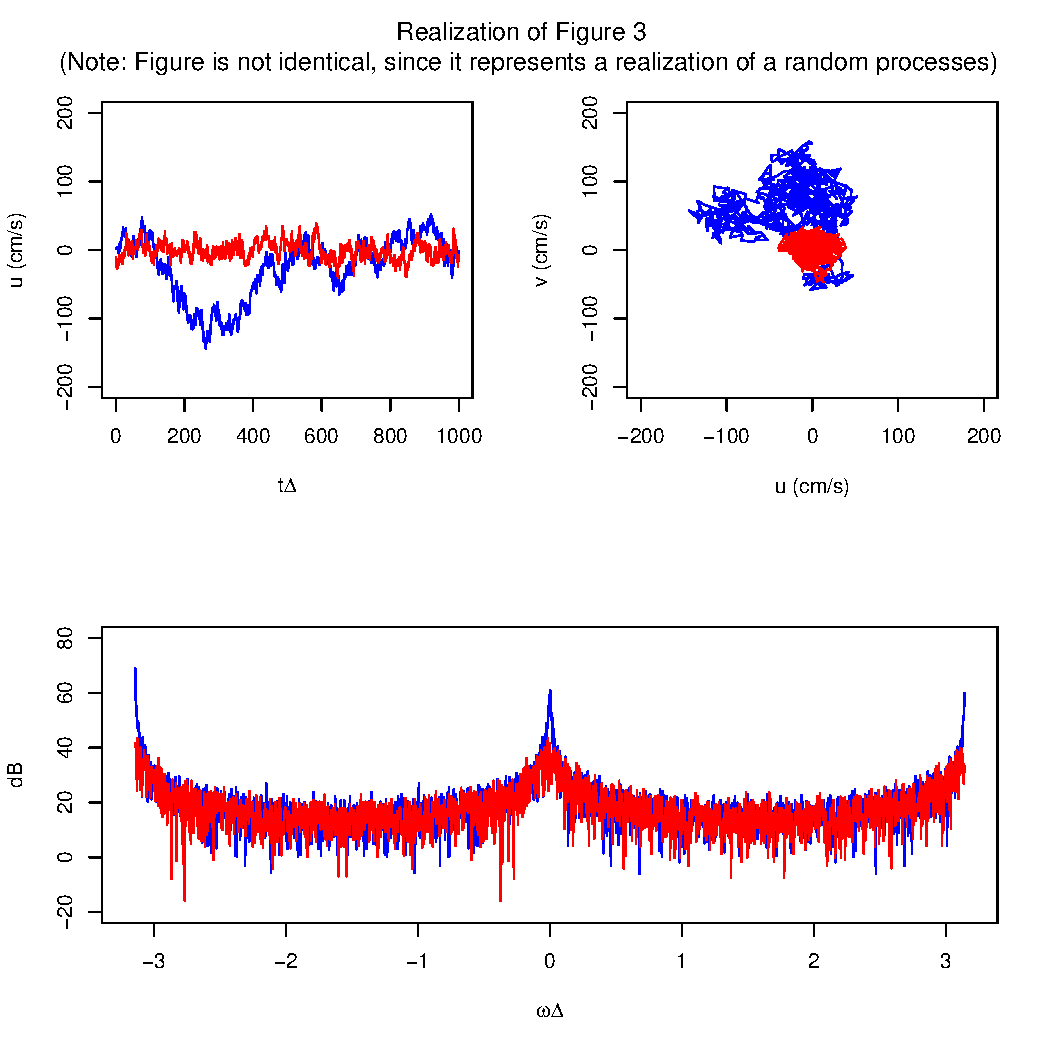
\includegraphics[width=.5\textwidth]{fig3.pdf}
        \caption{Simulated velocities obtained using FBM (blue) and Mat\'{e}rn (red)  processes. Top Left: The eastward component the velocity; Top Right: The eastward and northward components of the vecocity; Bottom: Periodograms on the decibel scale}
\end{figure}

\subsubsection{Overall Model}
Combining the inertial oscillation and turbulent background parts of the model is straightforward. To find both the autocovariance and power spectral densities, we can simply add the corresponding components of the inertial oscillation and turbulent background. Using Equations ~\ref{eq:ouAC} and ~\ref{eq:maternAC} and Equations ~\ref{eq:ouPSD} and ~\ref{eq:maternPSD}, we obtain
\begin{align}
S(\omega; \boldsymbol{\theta}) &= \frac{A^{2}}{(\omega - \omega_{0}) + c^{2}} + \frac{B^{2}}{(\omega^{2} + h^{2})^{\alpha}}\\
\label{eq: fullSpec}
s_{\tau}(\boldsymbol{\theta}) &= \frac{A^{2}}{2c} \exp(i \omega_{0}\tau) \exp(-c|\tau|) +  \frac{B^{2}}{2^{\alpha - 1/2}\pi^{1/2} \Gamma(\alpha) h^{2 \alpha - 1}}(h|\tau|)^{\alpha - 1}\kappa_{\alpha - 1/2}(h|\tau|).
\end{align}

\subsection{Fitting the Model}
\subsubsection{Blurred Whittle likelihood}
A new technique introduced in  \citet{Sykulski2013}  is used to fit the model. Referred to as \textbf{\it{blurred Whittle likelihood}}, this new likelihood builds on the well-known Whittle likelihood, a frequency-based approximation  to the time-domain likelihood that reduces computational cost.  Whittle likelihood is designed to approximate the likelihood for a univariate Gaussian process, $Z$,  in the time domain that has the likelihood
\begin{align*}
l_{t}(\theta) = - \frac{1}{2} log |C_{Z}(\theta) | - \frac{1}{2} Z^{T} C_{Z}^{-1}(\theta)Z
\end{align*}
where $\theta$ are the model parameters for a particular choice of covariance structure  and $t$ denotes the time domain  \citep{Sykulski2013}.  It is known that  the periodogram, given in Equation ~\ref{eq: perio}, satisfies
\begin{equation}
|J_{Z}(\omega)| \overset{d}{\rightarrow} S_{Z}(\omega) \chi^{2}_{2}/2
\end{equation}
under certain regularity conditions CITE. \citet{Whittle1953} combined this result with Fourier approximations to the true covariance structure and features of Toeplitz matrices to obtain the approximate likelihood
\begin{align}
l_{\omega}(\theta) &= - \sum_{\omega \in \Omega} \left[ J_{Z}^{H}(\omega) \tilde{S}_{Z}^{-1}(\omega; \theta) J_{Z}(\omega) + \log \{S(\omega; \theta) \} \right]\\
\label{eq: bwl}
&= -\sum_{\omega \in \Omega} \left[ \frac{\hat{S}_{Z}(\omega)}{S(\omega;\theta)}  + \log  \{ S(\omega; \theta) \}\right]
\end{align}
 where the subscript $w$ indicates that this is a Whittle likelihood and $H$ denotes a Hermitian matrix.  However, this likelihood relies on the periodogram and so is affected by aliasing and leakage as discussed in Section ~\ref{sec: specAnalysis}. 
 
To improve on these problems, \citep{Sykulski2013} propose replacing the theoretical spectrum, $S_{Z}(\omega; \theta)$ with the expected value of the spectrum, $\overline{S}_{Z}(\omega, \theta)$\begin{equation}
\overline{S}(\omega; \theta) = \Delta \sum_{\tau = - (N - 1)}^{N-1} \left(1 - \frac{|\tau|}{N} \right)s_{\tau}(\theta) exp ( - i \omega \tau \Delta)
\end{equation}
in Equation ~\ref{eq: bwl}. This form of the expected spectrum can be shown to be equivalent to convolving the theoretical spectrum with the Fe\'{j}er kernel 
\begin{equation}
\mathcal{F}(\cdot) = \frac{\Delta}{2\pi N} \frac{sin^{2}(N \omega \Delta/2)}{sin^{2}(\omega \Delta /2)} 
\end{equation} \citep{Sykulski2013}. This improves the estimators obtained through maximizing the likelihood, because the expected value of the periodogram $\mathbb{E}[|J_{Z}(\omega)^{2}]$ is blurred in the same way as the observed periodogram; thereby eliminating effects due to sampling at discrete intervals. This leads to the final likelihood
\begin{align}
l_{b}(\theta) = - \sum_{\omega \in \Omega} \left[\frac{\hat{S}_{Z}(\omega)}{\overline{S}(\omega; \theta)} + \log \{ \overline{S} (\omega; \theta) \}\right]
\end{align}
which is maximized by standard optimization techniques.

\subsubsection{Semi-parametric fitting}
The authors note that the fitting of Equation ~\ref{eq: fullSpec} can be adapted to reflect background knowledge about the drifters such as how the physical system behaves or artifacts from interpolation. They refer to these adaptations to the model as the semi-parametric approach and highlight its use  their analyses. Specifically,  variability can be different for the eastward versus northward velocities  which creates spurious correlations between positive and negative correlations. To avoid this, the authors only fit the model using data on the positive or negative half of the spectrum corresponding to the sign of the inertial oscillation ( which is known based on the latitude of the drifter).  Similarly, sampling effects make the accuracy of high frequencies suspect, so the authors only use frequencies up to a specified threshold in fitting the model. 

\subsubsection{Non-stationarity}
Further, to allow for non-stationarity in long time series, \citep{Sykulski2016} propose fitting the model independently at each observed time point using a rolling window around the time point of interest. This gives the OU differential equation
\begin{equation}
dz(t) = \{i \omega_{0}(t) - c(t) \} z(t) dt + A(t) dQ(t)
\end{equation}
and spectral power density
\begin{equation}
S^{(0)}(\omega, t) = \frac{A(t)^{2}}{\{\omega - \omega_{0}\}^{2} + c(t)^{2}}. 
\end{equation}
with parameters as a function of time. Similarly, the time-varying version of Mat\'{e}rn power spectral density is 
\begin{equation}
S^{(m)}(\omega, t) = \frac{B^{2}(t)}{\{\omega^{2} + h^{2}(t)\}^{\alpha(t)}}.
\end{equation}
The length of the window to fit these time-varying parameters needs to be large enough to allow for a full sampling of the spectrum, but short enough to be treated as locally stationary.  In this analysis, the authors select a reasonable window length empirically, but acknowledge that further work on this subject would be of value.  

\subsubsection{Significance tests for simpler models}
Finally, \citet{Sykulski2016} propose that a simple likelihood ratio test can be used at each time period to test whether or not a shift in the inertial oscillation has occurred. To do so, the authors suggest fitting a simpler model where the the parameter $\omega_{0}$ is fixed to be the inertial frequency $f$. Then this simpler model can be compared to the full six parameter model via a likelihood ratio test with test statistic
\begin{equation}
\label{eq: LRT}
R(t) = 2[l_{b} \{\hat{\theta}_{1}(t) \} - l_{b}\{\hat{\theta}_{0}(t) \} ]
\end{equation}
where $\hat{\theta}_{0}(t)$ is the fitted parameter vector for the simpler, or null model, and $\hat{\theta}_{1}(t)$ is the fitted parameter vector for the full model. The authors claim $R(t)$ then follow a Chi-Squared distribution with 1 degree of freedom.

\section{Results}
We show the potential utility of this method by analyzing two non-trivial data sets.  First, we consider the modeled trajectories of 200 near surface particles obtained from a computer simulation of ocean circulation (Set to be `very similar' to \citet{Danioux2008} SPEM 5.2 set-up). In Figure ~\ref{fig:numSim}, we display the fit of the aggregate spectral model to a single trajectory from the simulation and to an ensemble of trajectories. The resulting spectra has peaks at zero and at the inertial frequency, which indicates that the model captures the turbulent background and the inertial oscillations, which are set not to have shifts. We also display the individual periodograms and model fits. \citet{Sykulski2016}  note that this highlights the method's robustness, since the individual periodograms show considerable variability, but the model fits are all quite consistent.
\begin{figure}[hb]
	\label{fig:numSim}
  \centering
    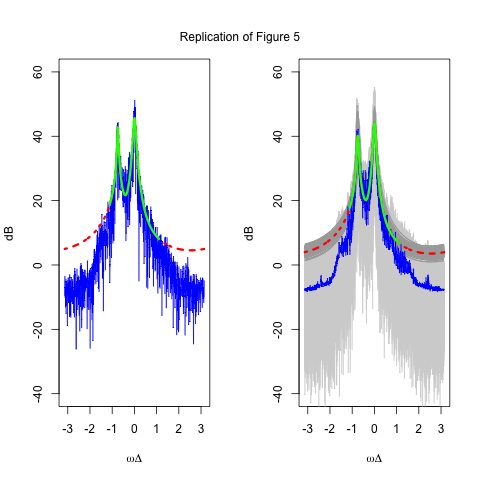
\includegraphics[width=.5\textwidth]{fig5.png}
        \caption{Left: The spectral density of one particle (blue) with the model fit overlaid for the portion of the spectra used to fit it (green) and extended to all frequencies (red). Right: The ensemble mean periodogram (blue) with the ensemble fit for the frequencies used to fit it (green) and extended to the entire spectrum (red) and individual trajectories' periodograms (light grey) and model fits (dark fit) }
\end{figure}

We also consider the trajectory of a drifter in the South Pacific Ocean observed 12 times a day over a 1642 day period. Using a rolling window of 1000 observations and the semi-parameteric set-up described in Section X, we obtain parameter estimates for the spectral model at each time point. In Figure ~\ref{fig:timeVarying}, we compare the observed spectral density over time and the fitted spectral density. The fitted density appears to be a smoothed version of the observed density, indicating a reasonable model fit. We also display the fitted parameter values over time and their 95$\%$ confidence interval bands in Figure 8 (add fig and renumber) and report the correlation among variables in Figure 10 (and fig and renumber). 

We also fit a 5-parameter where the frequency is set to the inertial frequency rather than being a free-parameter. We then compare the fit to the full model using a likelihood ratio test as described in Section X. In Figure 9, we display the test statistic over time where a red line is used to indicate the level of statistical significance. We conclude for time periods where the test statistic is greater than this cut-off that there is a shift in the inertial frequency. 


\begin{figure}[hb]
	\label{fig:timeVarying}
  \centering
    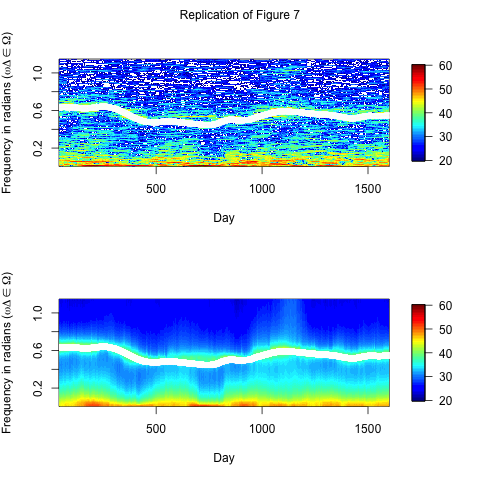
\includegraphics[width=.5\textwidth]{fig7.png}
        \caption{Top: Observed spectra of the drifter over time; Bottom: Modeled spectra over time. On both figures, the white line indicates the average inertial frequency within the rolling window at the current time period.  Only frequencies used in the estimation are included.  }
\end{figure}

\section{Discussion}
identifiability 



\clearpage

\bibliography{prelim}


\section{Appendix}

\subsection{Errata}

\subsection{Additional Figures}

\subsection{Computation}



\end{document}

